\documentclass[onecolumn,draftclsnofoot, 10pt, compsoc]{IEEEtran}

\usepackage{graphicx}
\usepackage[section]{placeins}
\usepackage{caption}

\usepackage{amssymb}                                         
\usepackage{amsmath}                                         
\usepackage{amsthm}                                

\usepackage{alltt}                                           
\usepackage{float}
\usepackage{color}
\usepackage{url}

\usepackage{balance}
\usepackage[TABBOTCAP, tight]{subfigure}
\usepackage{enumitem}
\usepackage{pstricks, pst-node}
\usepackage{url}
\usepackage{setspace}

\usepackage{etoolbox}
\AtBeginEnvironment{quote}{\singlespacing\vspace{-\topsep}\small}

%\input{pygments.tex}

\usepackage{geometry}
\geometry{left=0.75in,right=0.75in,top=0.75in,bottom=0.75in}
\parindent = 0.0 in
\parskip = 0.1 in


\def \ParSpace{\vspace{.75em}}
\def \GroupNumber{		17}
\def \Jeremy{			Jeremy Fischer}
\def \Class{		Parallel Programming}
\def \Assn{		Project 1: OpenMP: Numeric Integration with OpenMP}
\def \School{	Oregon State University}
\def \Professor{		Matthew Meyn}

\newcommand{\cred}[1]{{\color{red}#1}}
\newcommand{\cblue}[1]{{\color{blue}#1}}

\newcommand{\NameSigPair}[1]{
		\par
		\makebox[2.75in][r]{#1} \hfil 	\makebox[3.25in]{\makebox[2.25in]{\hrulefill} \hfill			
		\makebox[.75in]{\hrulefill}}
		\par\vspace{-12pt} \textit{
			\tiny\noindent
			\makebox[2.75in]{} \hfil		
			\makebox[3.25in]{
				\makebox[2.25in][r]{Signature} \hfill	\makebox[.75in][r]{Date}
			}
		}
}










%%%%%%%%%%%%%%%%%%%%%%%%%%%%%%%%%%%%%%%
\begin{document}
\begin{titlepage}
    \pagenumbering{gobble}
    \begin{singlespace}
    	
\includegraphics[height=4cm]{coe.eps}
        \hfill  
        \par\vspace{.2in}
        \centering
        \scshape{
            \vspace{.5in}
            \textbf{\Large\Assn}\par
            \textbf{\large\Class}\par
            \large{
            	\today \\Spring Term
        	}
            \vfill
            {\large Prepared for}\par
            \huge \School\par
            \vspace{5pt}
            {\Large{\Professor}\par}
            {\large Prepared by }\par
           % Group\GroupNumber\par
            \vspace{5pt}
            {\Large
                {\Jeremy}\par
            }
            \vspace{20pt}
        }

    \end{singlespace}
\end{titlepage}
\newpage
\pagenumbering{arabic}

% 7. uncomment this (if applicable). Consider adding a page break.
%\listoffigures
%\listoftables
\clearpage


	\section{Tell what machine you ran this on}	
	I ran this test on a 2015 Macbook Pro, 2.2 GHz Intel Core i7, 16 GB 1600 MHz DDR3.
	
	
	\section{What do you think the actual volume is?}
	I think the actual volume is 25.31. After plenty of testing with varying numbers of nodes, the volume converges to 25.31.
	
	
	\section{Show the performances you achieved in tables and graphs as a function of NUMNODES and NUMT}
	
	The below values are in mega (10\textsuperscript{6}) heights calculated per second.
	
	\begin{center}
		\begin{tabular}{|c| |c| |c| |c| |c|} 
			\hline
			\textit{Num Nodes} & \textit{1 Thread} & \textit{2 Threads} & \textit{4 Threads} & \textit{6 Threads} \\
			\hline
			
			\textbf{500} &	41.56	& 77.74	& 140.37	& 143.68 \\
			\hline
			
			\textbf{1000}	& 42.69	& 82.7	& 158.15	& 167.98
 \\
			\hline
			
			\textbf{3000}	& 40.79& 	81.73	& 146.87	& 172.41
 \\
			\hline
			
			\textbf{5000}	& 41.09	& 83.42	& 156.54& 	173.65
 \\
			\hline
			
			\textbf{7000}	& 36.39	& 82.8	& 155.61	& 175.35
 \\
			\hline
			
			\textbf{10000}	& 37.61	& 81.26	& 147.63	& 172.84
 \\
			\hline
			
			\textbf{15000}	& 38.53& 	79.42	& 146.81& 	176.31
 \\
			\hline
			
			\textbf{20000}	& 41.47	& 83.13	& 156.57& 	174.66 \\
			\hline
		\end{tabular}
	\end{center}
	
	\begin{figure}[t]
		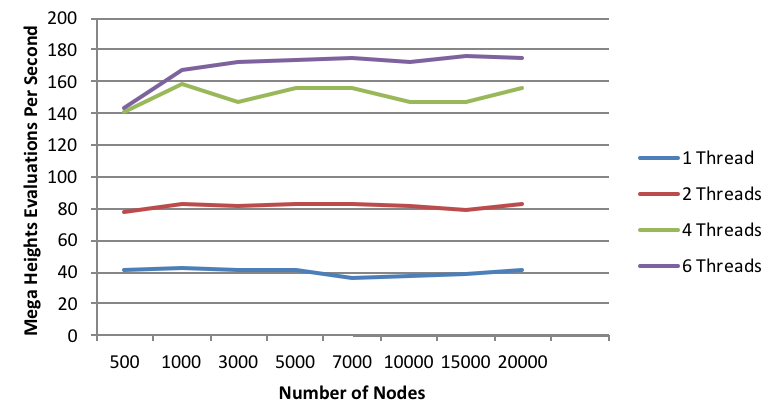
\includegraphics[width=18cm]{megasVnodes}
		\centering
	\end{figure}

	\begin{figure}[t]
		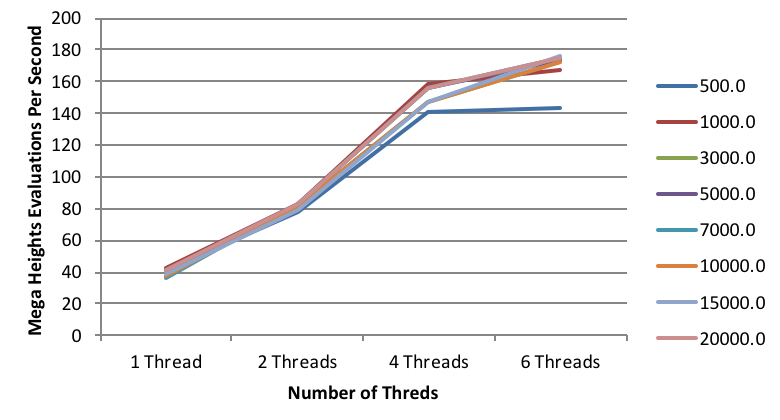
\includegraphics[width=18cm]{megasVthreads}
		\centering
	\end{figure}
	
	
	\section{What patterns are you seeing in the speeds?}
	The speed increases with each additional thread (as expected). However, the speed begins to increase less after the fourth thread. This is evident in the size of the gaps between the lines in the \textit{Mega Heights Evaluations Vs. Number of Nodes} graph below. The Plateau is also evident in the \textit{Mega Heights Evaluations Vs. Number of threads} graph. Between the fourth and the sixth thread there is a sharp cutoff.
	
	
	
	\section{Why do you think it is behaving this way?}
	The speedup associated with additional threads is due to the OMP reduction in calculating the \textit{dV'}s. Each thread claims a portion of the tiles and computes the total volume of their section. When all threads are done, the real total volume is calculated by computing the summation of each individual thread's calculated volume .
	
	I think that the plateau in the speed increase is due to Amdahl's law. Essentially, there comes a point where increasing the number of threads doesn't improve the speed by the same magnitude as the previous thread.
	
	
	
	
	\section{What is the Parallel Fraction for this application, using the Inverse Amdahl equation?}
	Using the Inverse Amdahl equation and the Speedup equation where T1 and T6 are in nanoseconds, the Parallel Fraction for this application is \dots
	
	\[Speedup = \frac{T1}{T6} = \frac{5355766000.226140}{1297830000.519753} =  4.126\]
	
	\[F_{parallel} = \frac{n}{n-1} (1 - \frac{1}{Speedup}) = \frac{6}{5} (1 - \frac{1}{4.126}) = 0.910\]
	
	
	
	
	\section{Given that Parallel Fraction, what is the maximum speed-up you could ever get?}
	Using the Parallel Fraction = 0.910, the maximum speedup you could ever get is \dots
	
	\[ Max Speedup = \frac{1}{1 - F_{parallel}} =  \frac{1}{1 - 0.910} = 11.11\]

	

	
	



\end{document}